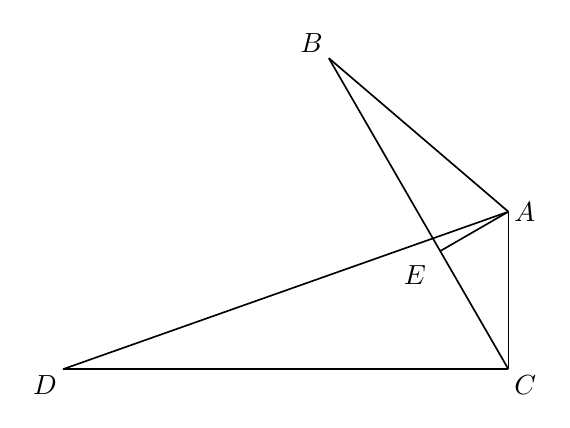
\begin{tikzpicture}[x=1cm,y=1cm,font=\normalsize,
 geometry edge/.style={solid,line width=.6pt},
 geometry mark/.style={solid,line width=.6pt},
 geometry label/.style={font=\normalsize,inner sep=2pt}]
\coordinate (C) at (0,0);
\coordinate (A) at (0,2);
\coordinate (D) at (-5.656854249,0.000000000);
\coordinate (E) at (-0.866025404,1.500000000);
\coordinate (B) at (-2.280238966,3.949489743);
\draw[geometry edge] (D)--(C);
\draw[geometry edge] (C)--(A);
\draw[geometry edge] (D)--(A);
\draw[geometry edge] (B)--(E);
\draw[geometry edge] (E)--(C);
\draw[geometry edge] (B)--(A);
\draw[geometry edge] (A)--(E);
\node[geometry label,below right] at (C) {$C$};
\node[geometry label,right] at (A) {$A$};
\node[geometry label,below left] at (D) {$D$};
\node[geometry label,below left,xshift=-3pt,yshift=-3pt] at (E) {$E$};
\node[geometry label,above left] at (B) {$B$};
\end{tikzpicture}
